\documentclass[12,twoside]{TFG-GM}
%\usepackage[active]{srcltx}
\usepackage{amsthm,amsmath,amssymb,amsfonts,amscd}
\usepackage{graphicx}
\usepackage{enumerate}
\usepackage[all]{xy}
\usepackage{booktabs}
%\usepackage[usenames]{xcolor}
%\usepackage{fancyhdr}

%%%%%Author packages if necessary


% Theorem Environments: add extra ones at the end if you need it.

\newtheorem*{theoremA}{Theorem A}
\newtheorem{theorem}{Theorem}[section]

\newtheorem{proposition}[theorem]{Proposition}
\newtheorem{lemma}[theorem]{Lemma}
\newtheorem{corollary}[theorem]{Corollary}
\newtheorem{conjecture}[theorem]{Conjecture}

\theoremstyle{definition}
\newtheorem{definition}[theorem]{Definition}
\newtheorem{example}[theorem]{Example}

\theoremstyle{remark}
\newtheorem{remark}[theorem]{Remark}
\newtheorem*{remarknonumber}{Remark}
\newtheorem{observation}[theorem]{Observation}




%%%%%%%%%%%%%%%%%%
% macros/abbreviations: Include here your own.
%%%%%%%%%%%%%%%%%%

\newcommand{\N}{\ensuremath{\mathbb{N}}}


% Body of document

\titol{A learning approach\\[3mm] to the FOM problem}
\titolcurt{A learning approach to the FOM problem}
\authorStudent{Eudald Romo Grau}
\supervisors{Alberto Rodriguez Garcia and Maria Alberich Carrami\~nana}
\monthYear{April, 2017}

%\msc[2010]{Primary  	55M25, 57P10, Secondary 55P15, 57R19, 57N15.}

\paraulesclau{Manipulation, Online Control, MPC, FOM, Underactuation, Hybridness}
\agraiments{
Thanks to Alberto Rodriguez for his tutoring, for providing me with the required tools and financial support to undertake this project and for hosting me in his laboratory, to Maria Alberich for her supervision and tutoring, to Francois Hogan for his ideas and the introduction he gave me to his previous work, to Maria Bauza for her insights in Machine Learning, to all the members of the MCube Lab for their thoughts on the project and their support, to Centre de Formacio Interdisciplinaria Superior for offering me the possibility and the financial support to take part in this project, to Massachusetts Institute of Technology for providing the required facilities required to develop this project and to Generalitat de Catalunya for their financial support.}


\abstracteng{The family of modes (FOM) approach to solving model predictive control (MPC) problems is a novel heuristic technique developed at MIT to solve the time complexity of traditional MPC solving techniques. This study addresses some of the issues associated with the previous formulations of this technique by increasing the sequential robustness of the FOM and providing methodologies to choose the parameters required for the heuristic. A general simulation interface is developed together with techniques to score and compare the obtained trajectories. Then an statistics and machine learning based methodology is developed to tune the parameters is proposed and the results are compared with the original ones. Finally, experimental procedures are developed to validate the results.}

%%%%%%%%%
\begin{document}

\maketitle

\section{Introduction}
\label{sec:intro}
Recently, there has been a lot of progress in the worlds of manipulation and locomotion. ADD SOME EXAMPLES HERE.

Complementarity constraints led to hybrid state formulations. MPC allowed to convexify those formulations. MPC grows exponential with the number of  lookahead time steps.

Feedback is hard/requires effort. All the teams in the ARC used open loop systems (as of the 2nd edition of the competition) [add reference]

Feedback is important. Robots fall because control in hybrid systems still has a long way to go.


This allowed to tackle problems as state hybridness (ADD COMPLEMENTARITY CONSTRAINTS AND HYBRID PROBLEMS). This allowed further progress into the planning branch of these problems. Unluckily, the complexity of the traditional formulations for these problems requires discretization of the time space of the problem and the algorithmic cost of the used solvers usually grows exponentially with the number of considered time steps. This has been translated into a relatively lower progress of the correspondent online control branch.

\subsection{Prior Work}
\label{subsec:priorWork}

\subsection{Complementarity Constraints}
\label{subsec:Complementarity Constraint}
The Complementarity constraint formulation [TODO: INSERT REFERENCES] presented a formulation of hybrid problems that allowed to 

\subsection{Model Predictive Control}
\label{subsec:MPC}
One of the most common techniques 

\subsection{Family of Modes}
\label{subsec:FOM}
I have to talk about close loops and about manipulation. Then MPC, then first approach to the family of modes

En referencia al treball. Com et vaig dir, treballo estudiant les families de modes que el meu company va utilitzar al seu article. El problema que intenten solucionar es el de controlar una trajectoria hibrida en el pla. Tenim un dit que empeny el quadrat metal.lic que et vaig comentar i ha d'intentar que segueixi trajectories previament calculades. Com que en cada iteracio el sistema esta en un i nomes un dels tres possibles estats (adherencia, lliscament en una direccio o en l'altra) i cada estat te les seves propietats fisiques, que previament linearitzem. La manera naif de solucionar-ho seria crear un problema de Programacio lineal o quadratica per cada possible combinacio d'estats present a una trajectoria. El nombre de problemes que s'han de solucionar creix exponencialment. La manera tradicional de trencar l'exponencialitat es modelar cada iteracio amb les variables necessaries per descriure el sistema mes una variable entera (0 o 1) per cada possible estat. Aleshores simplement es formula el problema com un problema de Programacio Entera Mixte (MIP) i es soluciona amb algun programa especialitzat com ara Gurobi. Plantejar-ho com un MIP fa que, tot i que en el cas pitjor, el problema sigui sent exponencial en el nombre de variables, els metodes de programacio lineal que s'utilitzen per solucionar-ho (principalment Branch and Bound o Branch and Cut amb certes heuristiques) fan que el temps esperat sigui molt menor.

Es pot representar el conjunt de possibles problemes de programacio lineal que s'han de resoldre a traves d'un arbre. Cada node representa un dels tres estats possibles. L'arrel de l'arbre es un node buit i a cada pas de la trajectoria l'arbre es ramifica 3 nodes (un per cada possible estat). Cada cami des de l'arrel fins a una de les fulles defineix de manera unica un problema a solucionar. La solucio que nosaltres proposem es basicament una heuristica que nomes explora un conjunt limitat d'aquests camins i elegeix el millor. El problema que solucionem es un problema de control, no de planificacio, per tant, un cop obtenim una solucio, obtenim els valors que hem de passar al controlador per executar el primer pas, l'executem, obtenim la informacio necessaria a traves de sensors per determinar la nova nostra posicio i tornem a executar l'algorisme. Aixo ens permet reaccionar a perturbacions externes o a errors d'execucio (per exemple, podriem estar esperant que en un pas el dit robotic es mantingues adherit, pero el coeficient de friccio pot ser diferent a la zona on esta en aquell moment i lliscar en comptes de mantenir-se adherit). Per tant, el que fem es solucionar el problema un problema amb un horitzo reduit repetidament a una alta frequencia (solucionar el problema en tot moment des de la posicio actual fins al desti final acostuma a ser massa costos i no es pot fer a la frequencia necessaria). Aquest metode obte solucions suboptimes, pero esta motivat pel fet que la solucio del problema tradicional (MIP) no esta repartida homogeniament entre el conjunt de camins de l'arbre de decisions, hi ha alguns camins que son molt mes comuns que d'altres. L'objectiu ultim d'aquesta linia d'investigacio es obtenir resultats el mes propers possible a l'optim utilitzant un grup el mes reduit possible de camins.

En el moment d'arribar al laboratori em vaig trobar que el metode tenia encara defectes importants i requeria investigacio en algunes direccions. Un dels defectes era el fet que en cada iteracio nomes s'executes el primer pas de la trajectoria obtinguda. Aixo feia que la immensa majoria de families de camins fossin, a efectes practics, inutils. Per mostrar un exemple senzill, es pot considerar el cas en que la familia conte dos camins de tres iteracions, per exemple:
$$cami1 = {adherencia, lliscar_amunt, adherencia} i cami2 = {adherencia, lliscar_avall, adherencia}$$. Encara que entre els dos camins es tingui en compte la totalitat dels estats possibles, el dit robotic mai lliscara, ja que el primer pas dels dos camins es adherencia, i el controlador nomes executa el primer pas. Vaig estar mirant maneres de solucionar aquest problema i, si es volien mantenir camins estatics (es a dir, executar sempre els mateixos camins en cada iteracio), el nombre de camins necessaris tambe creixa molt rapidament, ja que per cada cami, hauries d'afegir totes les possibles translacions periodiques del cami.
Vaig considerar camins dinamics i vaig obtenir dues possibles solucions. La primera era principalment imaginar els camins com a camins periodics i traslladar-los una posicio al final de cada iteracio.
La segona era afegir un mode camaleo, que en cada iteracio simules la continuacio del cami seleccionat com a solucio de la iteracio anterior.

Les parts que requereixen investigacio son principalment les referents a la seleccio dels camins que a considerar i a la quantificacio del cami obtingut. Al moment d'arribar no hi havia cap manera establerta de decidir si un cami era millor que un altre. De moment he decidit utilitzar mateixos costos que s'utilitzen localment per solucionar els problemes de programacio lineal en l'horitzo reduit per evaluar la solucio total, ja que aixo em permet garantir alguns resultats teorics, com ara que, a part d'errors numerics al solucionar el MIP, la solucio del MIP ha de ser millor que la de la familia de modes.

Aquests ultims mesos he estat programant un codi en MATLAB per simular els dos metodes (familia de modes i MIP) basant-me en el codi anterior del meu company de laboratori. Ell tenia un codi prototip per solucionar un cas molt concret: familia de modes amb tres camins de 35 iteracions que segueix una linia recta. Ho he reestructurat tot per tal que es puguin generar camins arbitraris que combinin els estats que jo defineixi i seguir trajectories arbitraries. Aixo ha de permetre, per una banda, extendre el problema a casos mes complexos (trajectories mes complexes, un dit que pugui cambiar la cara del cub que empeny, multiples dits que empenyin diferents cares, etc). Per altra banda, la flexibilitat de generacio de camins i la implementacio del cost de la trajectoria final obtinguda ha de permetre estudiar la dependencia de la qualitat de la solucio obtinguda en funcio dels camins base seleccionats. Aixo obre la porta a aplicar tecniques d'aprenentatge per seleccionar els camins base per solucionar un cert problema.

A dia d'avui, el codi base esta practicament completat. Es poden seguir trajectories rectilinies o circulars i es pot quantificar la solucio obtinguda i mostrar-la en un video. En els propers dies provare la millora entre utilitzar o no el mode camaleo amb diferents seleccions de camins base. El proper pas sera utilitzar algun algoritme aleatori (alguna cosa similar a un algoritme genetic) per intentar millorar la seleccio de camins base. Aquest estudi inicial, encara que no proporcioni una manera formal d'aconseguir camins inicials, possiblement permeti tenir una nocio de la correlacio entre camins de la familia.

Et seguire informant de futures direccions en la investigacio. Tambe t'adjunto un video on es veu una simulacio amb familia de modes on s'intenta seguir una trajectoria circular objectiu (quadrat vermell). La trajectoria simulada (quadrat blau) te unes condicions inicials lleugerament perturbades.

This is an example of a document using the TFG-GM.cls document class. The TFG-GM.cls document class is a modification of the Reports@SCM class with minor differences (cover page, title colors and format for references) to facilitate the submission of your work to the journal Reports@SCM.

If your plan is submitting your work to the \textbf{journal Reports@SCM}, please note that:
\begin{itemize}
	\item The length of the core of the document should not exceed 10 pages, see the Reports@SCM web page for details.
	\item Further developments, explanations, codes or results are expected to be also included in this document as appendixes.
	\item You should not add any extra packages unless you consider it very necessary. See Section \ref{packages} to see which standard packages  are considered by default. 
\end{itemize} 

If you do not plan submitting your work to the journal  Reports@SCM, you can use this document as an example. \textbf{Using this template is not mandatory}.
 
In any case, \textbf{you must use the template for the main cover page} \texttt{coverMAMMEmasterThesis.doc} as explained in section \ref{sec:coverPage}.


\section{Adding the MAMME cover page to your document}
\label{sec:coverPage}
  
Regardless of the structure of the document of your TFG, you have to use the template \texttt{coverTFG-GM.doc} for the cover page. You can follow the fowolling steps:
\begin{itemize}
	\item Generate a pdf file with the document of your TFG, following or not this template
	\item Modify the document \texttt{coverTFG-GM.doc} with the data of your thesis and generate a pdf with two pages (cover and blank page)
	\item Use Adobe or other sofware to join (combine or merge) the two pdf files in one pdf file. 
\end{itemize}
 
\section{Environments}

In this section you can see examples of different environments.

\subsection{Theorem-like environments}

\begin{theorem} \label{th:example}
This is an example of a theorem, numbered with the section number.
\end{theorem}

\begin{proposition}
This is a proposition, numbered the same way. You can reference theorems and propositions using the labels, see for instance Theorem \ref{th:example}.
\end{proposition}

\begin{lemma}
This is a lemma, numbered the same way.
\end{lemma}

\begin{corollary}
This is a corollary, numbered the same way.
\end{corollary}

\begin{conjecture}
This is a conjecture, numbered the same way.
\end{conjecture}

If you need any other environment, you can add it to the preamble following the examples.

%%%%
\subsection{Definition-like environments}

\begin{definition}
This is a definition. Notice that the style is different than in theorems.
\end{definition}

\begin{example}
This is an example. Same style as definitions.
\end{example}

%%%%
\subsection{Remark-like environments}

\begin{remark}
This is a remark. 
\end{remark}

\begin{remarknonumber}
This is a remark with no numbered label. You may create other environments with no numbered label by copying from this example.
\end{remarknonumber}

%%%%%
\section{Figures}

Please include figures using the graphics package uploaded.  Fancy options can be found for example in  \begin{verbatim} http://www.kwasan.kyoto-u.ac.jp/solarb6/usinggraphicx.pdf \end{verbatim}

\begin{figure}[htb!]
\begin{center}
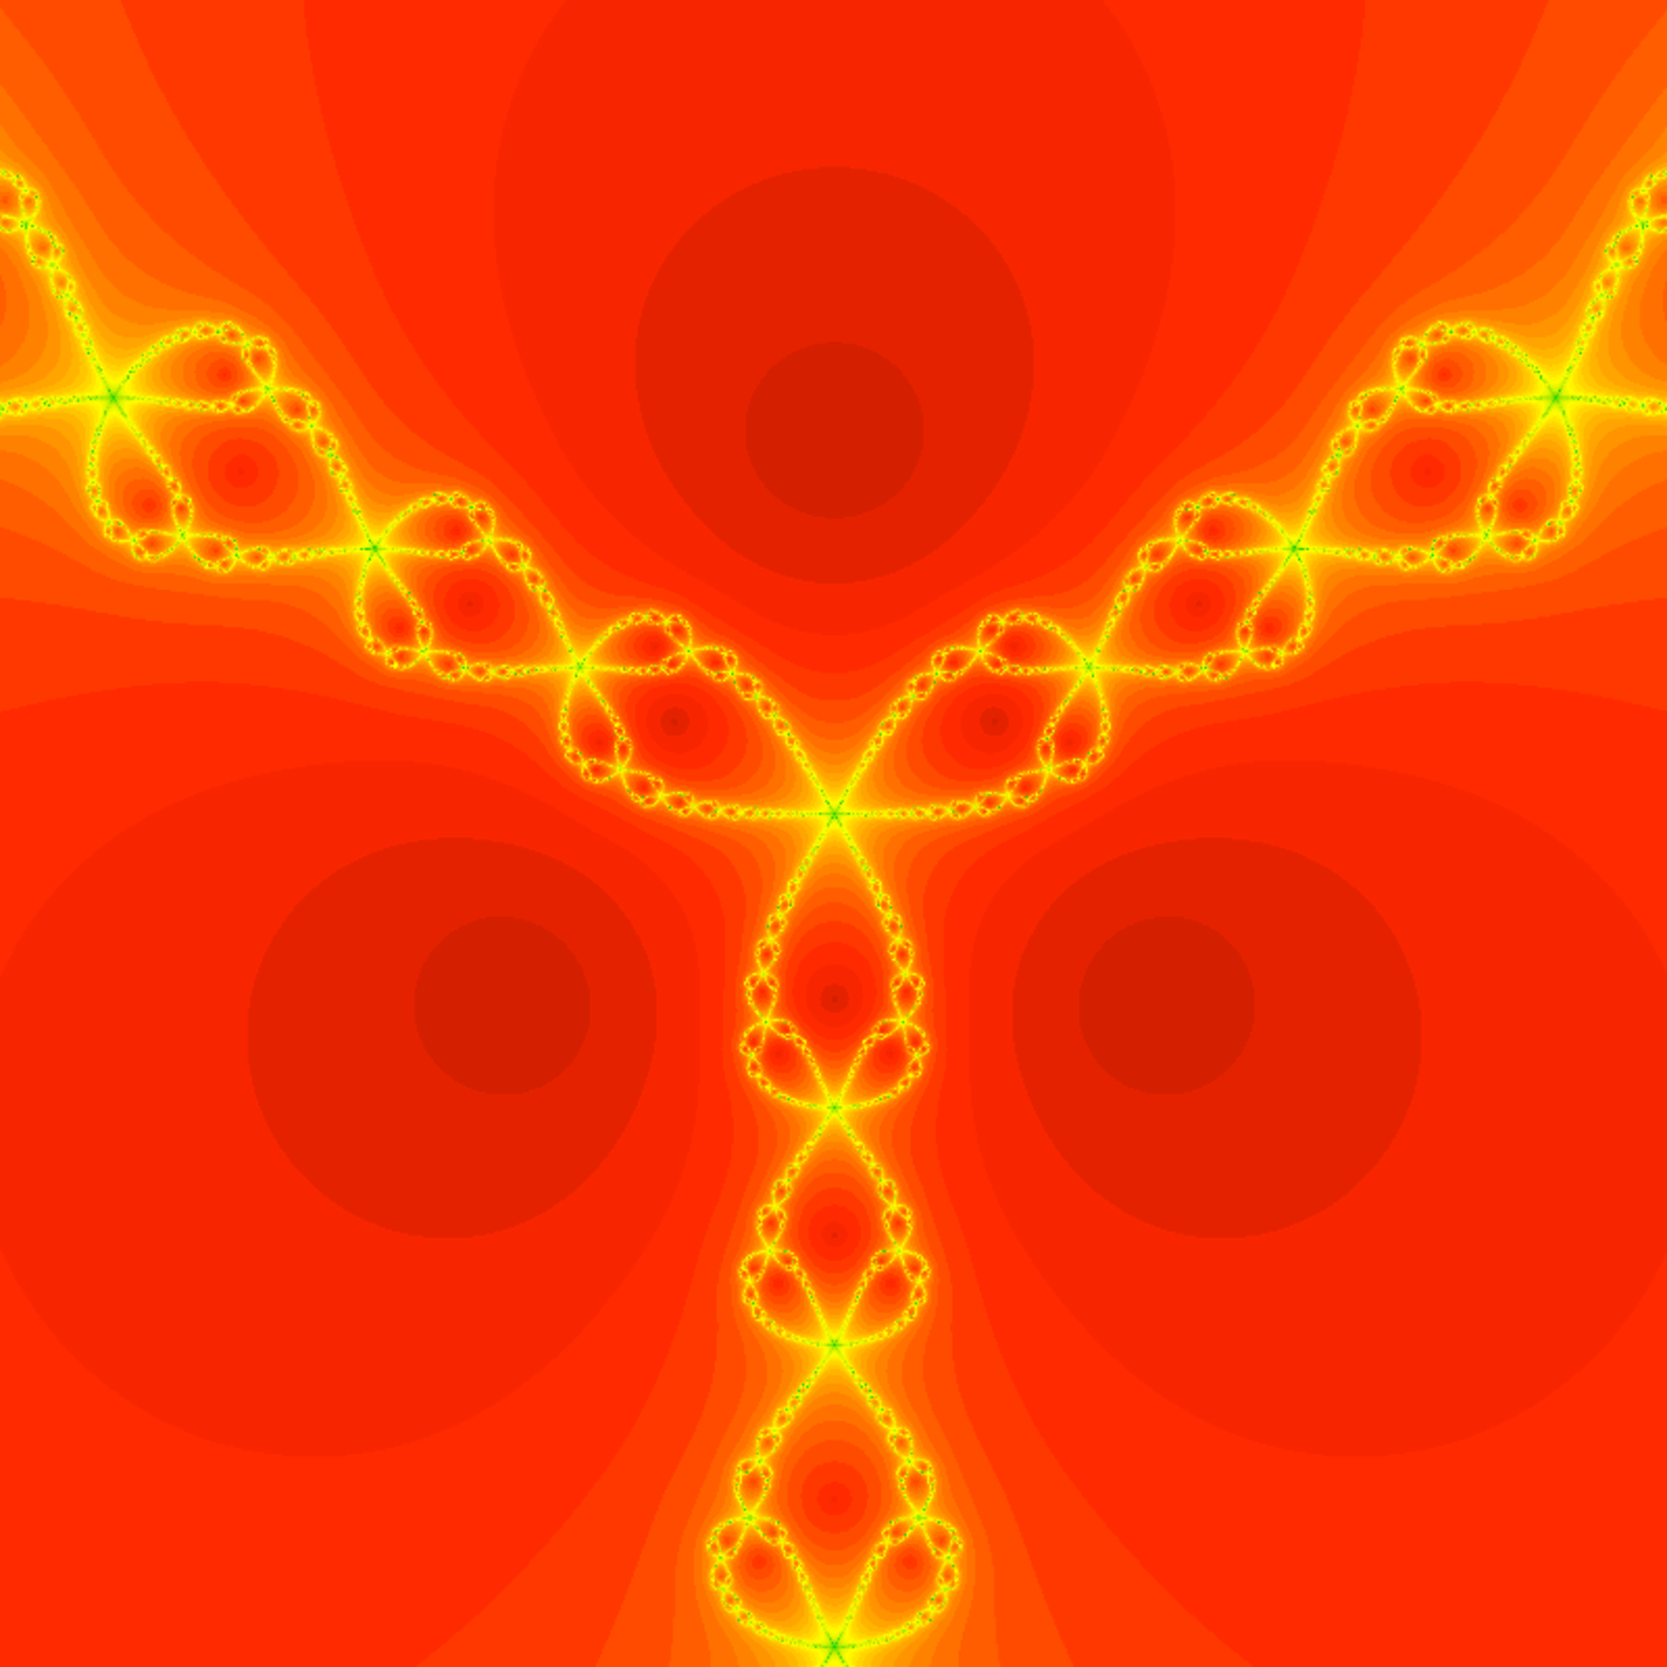
\includegraphics[width=6cm]{samplefigure.pdf}
\end{center}
\caption{\label{sample figure} \small The caption of this figure is ``Newton's method of a cubic polynomial".}
\end{figure}

%%%%%%%%
\section{Mathematics and packages} \label{packages}

By default, the following packages are uploaded:
\begin{enumerate}[\bf (1)]
\item {\tt enumerate:} It allows you to make list with specific somehow arbitrary labels, like this one.
\item {\tt amsthm:} To make evironments with different styles.
\item {\tt amsmath,amssymb,amsfonts:} Multiple mathematics symbols and fonts.
\item {\tt graphicx:} To include figures in a simple and intuitive way.
\item {\tt amscd:} To make commutative diagram with horizontal and vertical arrows. See below.
\item {\tt xy:} To make really fancy commutative arrows. See below.
\item {\tt booktabs:} To make fancy tables.
\end{enumerate}
You may add other standard packages if you need them but try to avoid it if at all possible.

If you need to use them, you will find information about these packages in the usual internet places. 

Here are examples of two commutative diagrams, one made with the package amscd and the other one with xy.

\[
\begin{CD}
A @>g>> B\\
@VV\pi V @VV\pi V\\
X @>f>> Y
\end{CD}
\]


\section{Bibliography}

You may include your references by hand using {\tt the bibliography} (see an example below) or, alternatively, you may use a .bib file and use BibTeX. In any case, we ask you to use a reasonable {\bf consistent} format for all your references. Our recommendation is using BibTex with the style   "plain" or "amsalpha".

%\newpage

\begin{thebibliography}{99}

\bibitem{ex} S.K.\,Agrawal, J.\,Yan. `A three-wheel vehicle with
    expanding wheels: differential flatness, trajectory planning, and control',
    \textit{Proc. of the 2003 IEEWRSJ, Intl. Conference on Intelligent Robots and
    Systems}, Las Vegas, 2003.

\bibitem{ah0} L.~Ahlfors. {\em Complex analysis. An introduction to the theory of analytic functions of one complex variable}, 3rd ed. McGraw-Hill, 1978.

\bibitem{ahl} L.~Ahlfors. {\em Lectures on quasiconformal mappings}, 2nd ed.
University Lecture series {\bf 38}, American Mathematical Society, 2006.

\bibitem{ahlber} L.~Ahlfors and L.~Bers.
  Riemann mapping's theorem for variable metrics,
{\em Annals of Math.}~{\bf 72} (1960), 385--404.
    
\bibitem{CLM89} B.\,Charlet, J.\,L\'evine, R.\,Marino. On dynamic feedback
    linearization, {\em System and Control Letters} \textbf{13} (1989), 143--151.

\end{thebibliography}

%______________________________________________________________
\appendix
\vfill\newpage \section{Title of the appendix}
You can include here an appendix with details that can not be included in the core of the document. You should reference the sections in this appendix in the core document.
\vfill\newpage \section{Title of the appendix}
Second appendix.

\end{document}


